\section{Chronik der parallelen Algorithmenentwicklung}
Parallele Verfahren finden nicht nur in der Algorithmik und Informatik allgemein Anwendung, sondern sind im täglichen Leben zu finden. Sobald mehrere Personen oder Maschinen parallel an der Lösung eines Problems oder Erstellung eines Gegenstandes (z.B. Autobau, Konstruktion von Gebäuden, etc.) arbeiten, ist dies ein paralleles Verfahren.\\
In der Informatik basierte lange Zeit jeder Computer auf der Von-Neumann-Architektur, d.h. es gab eine einzelne CPU. Damit waren sequentielles Arbeiten und somit auch sequentielle Algorithmen erzwungen. Parallelität gab es nur innerhalb der CPU durch verschiedene Schaltkreise, die nebeneinander arbeiten.\\
In Algorithmen und Programmierung ist die Idee paralleler Algorithmen schon seit den $1960\text{er}$ Jahren vorhanden und z.B. in den Büchern von Knuth zu finden.\\
In den $1980\text{er}$ und frühen $1990\text{er}$ Jahren wurde viel in dem Gebiet der parallelen Algorithmen und Architekturen geforscht und gearbeitet. Damals kam die Idee auf, anwendungsspezifische (special-purpose) parallele Architekturen zu entwickeln. Dazu wurden mehrere Prozessoren auf Gitterpunkten oder Kreisen angeordnet und auf bestimmte Art und Weise untereinander verbunden.\\ \\
{\bf{Beispiel (Hyperwürfel von Prozessoren):}} Die Prozessoren befinden sich auf den Gitterpunkten und sind mit den Nachbarn nach Vorschrift eines $d$-dimensionalen Würfels verbunden:
\\
\begin{figure}[h!]
\centering
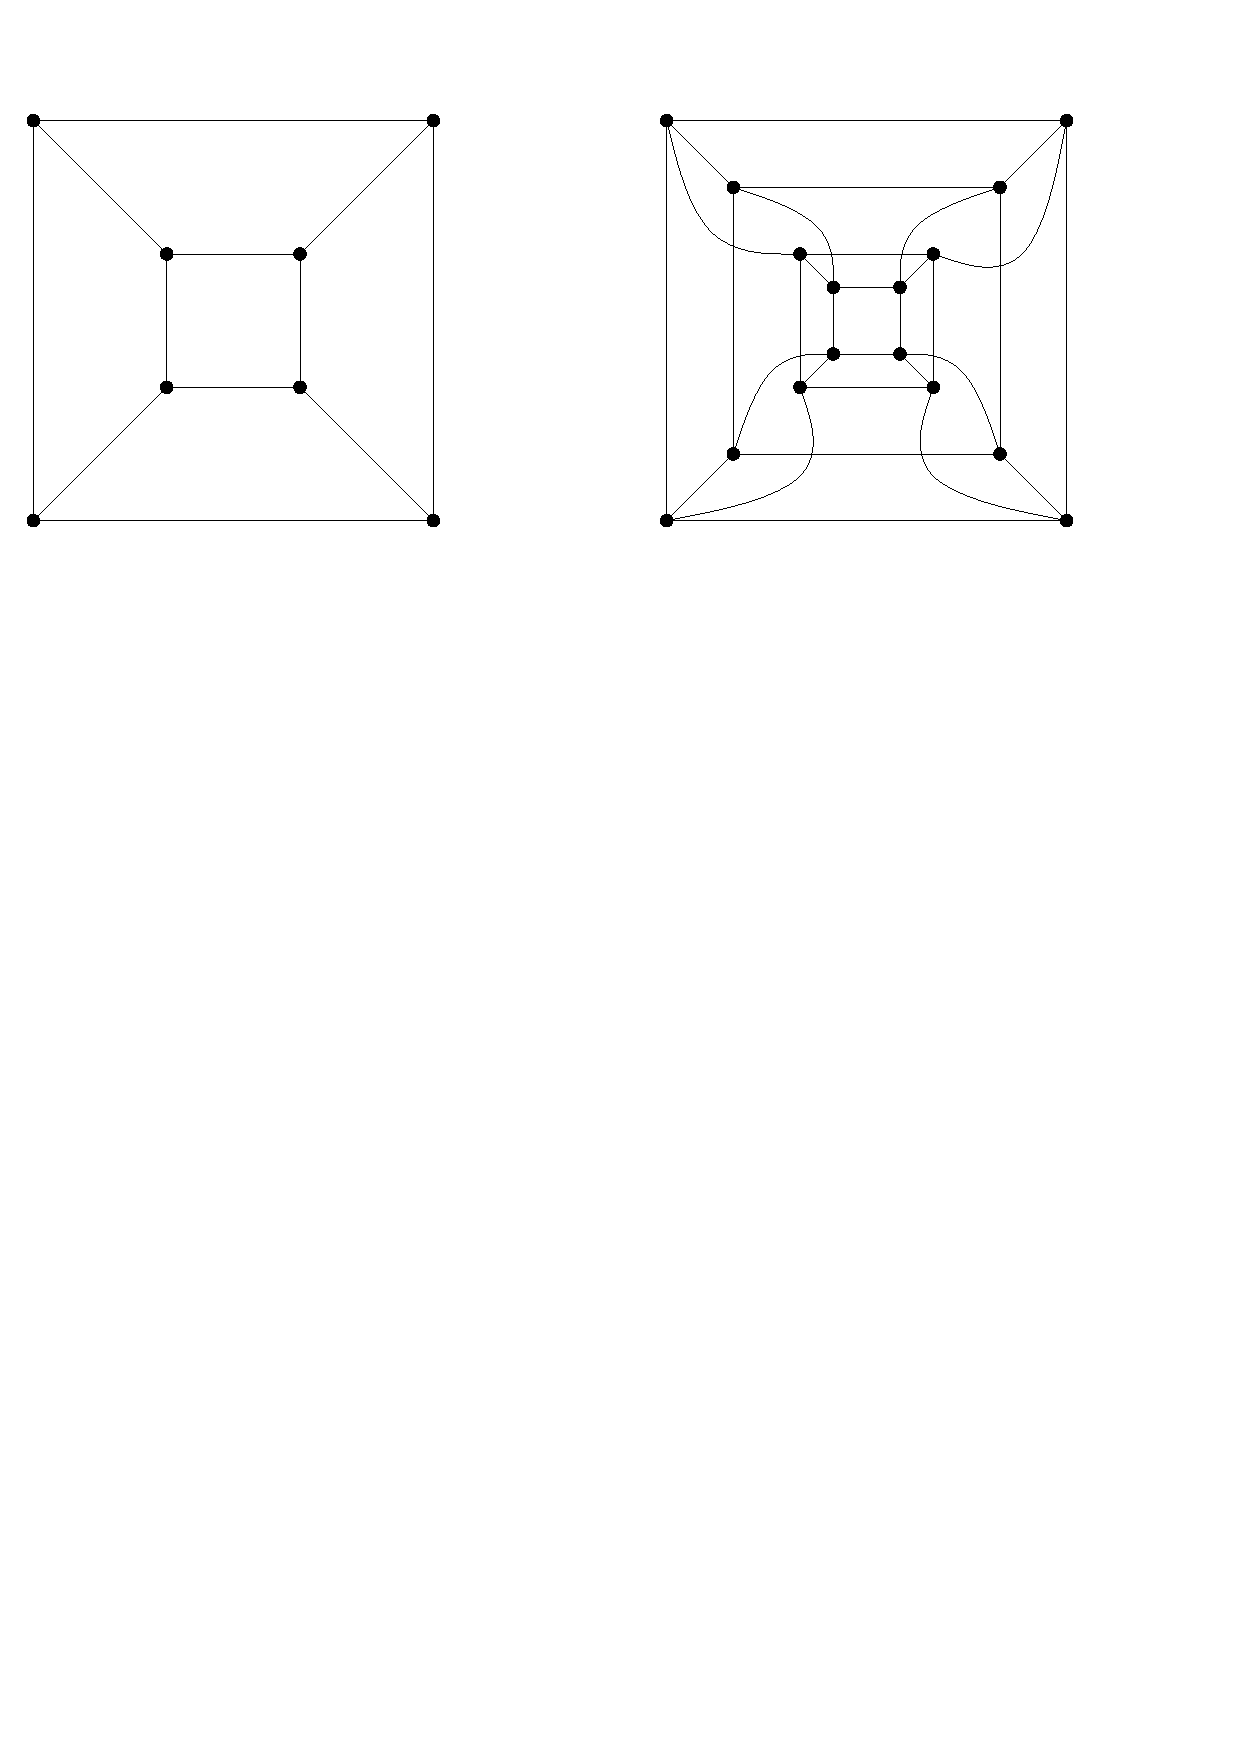
\includegraphics[scale=0.6]{bilder/Hyperwuerfel.pdf}
\caption{Drei- und vierdimensionaler Hyperwürfel}
\end{figure}

{\bf{Beispiel (Connection Machines):}}
Die Connection Machine CM1 bestand aus $65536$ $1$-Bit Prozessoren, die in der Art eines 16-dimensionalen Würfels angeordnet waren. Die Software war an der funktionalen Sprache LISP ausgerichtet.
\\
\\
Um parallele Algorithmen analysieren und vergleichen zu können wurde ein paralleles Berechnungsmodell entwickelt. Dieses theoretische Modell ist eine Weiterentwicklung der RAM und wird als parallele RAM (PRAM) bezeichnet.
\\
Eine parallele Registermaschine (PRAM) besteht aus einer Menge von Prozessoren, einem gemeinsamen Speicher und einem Befehlssatz. Die Prozessoren kommunizieren über den gemeinsamen Speicher miteinander.
\begin{figure}[h!]
\centering
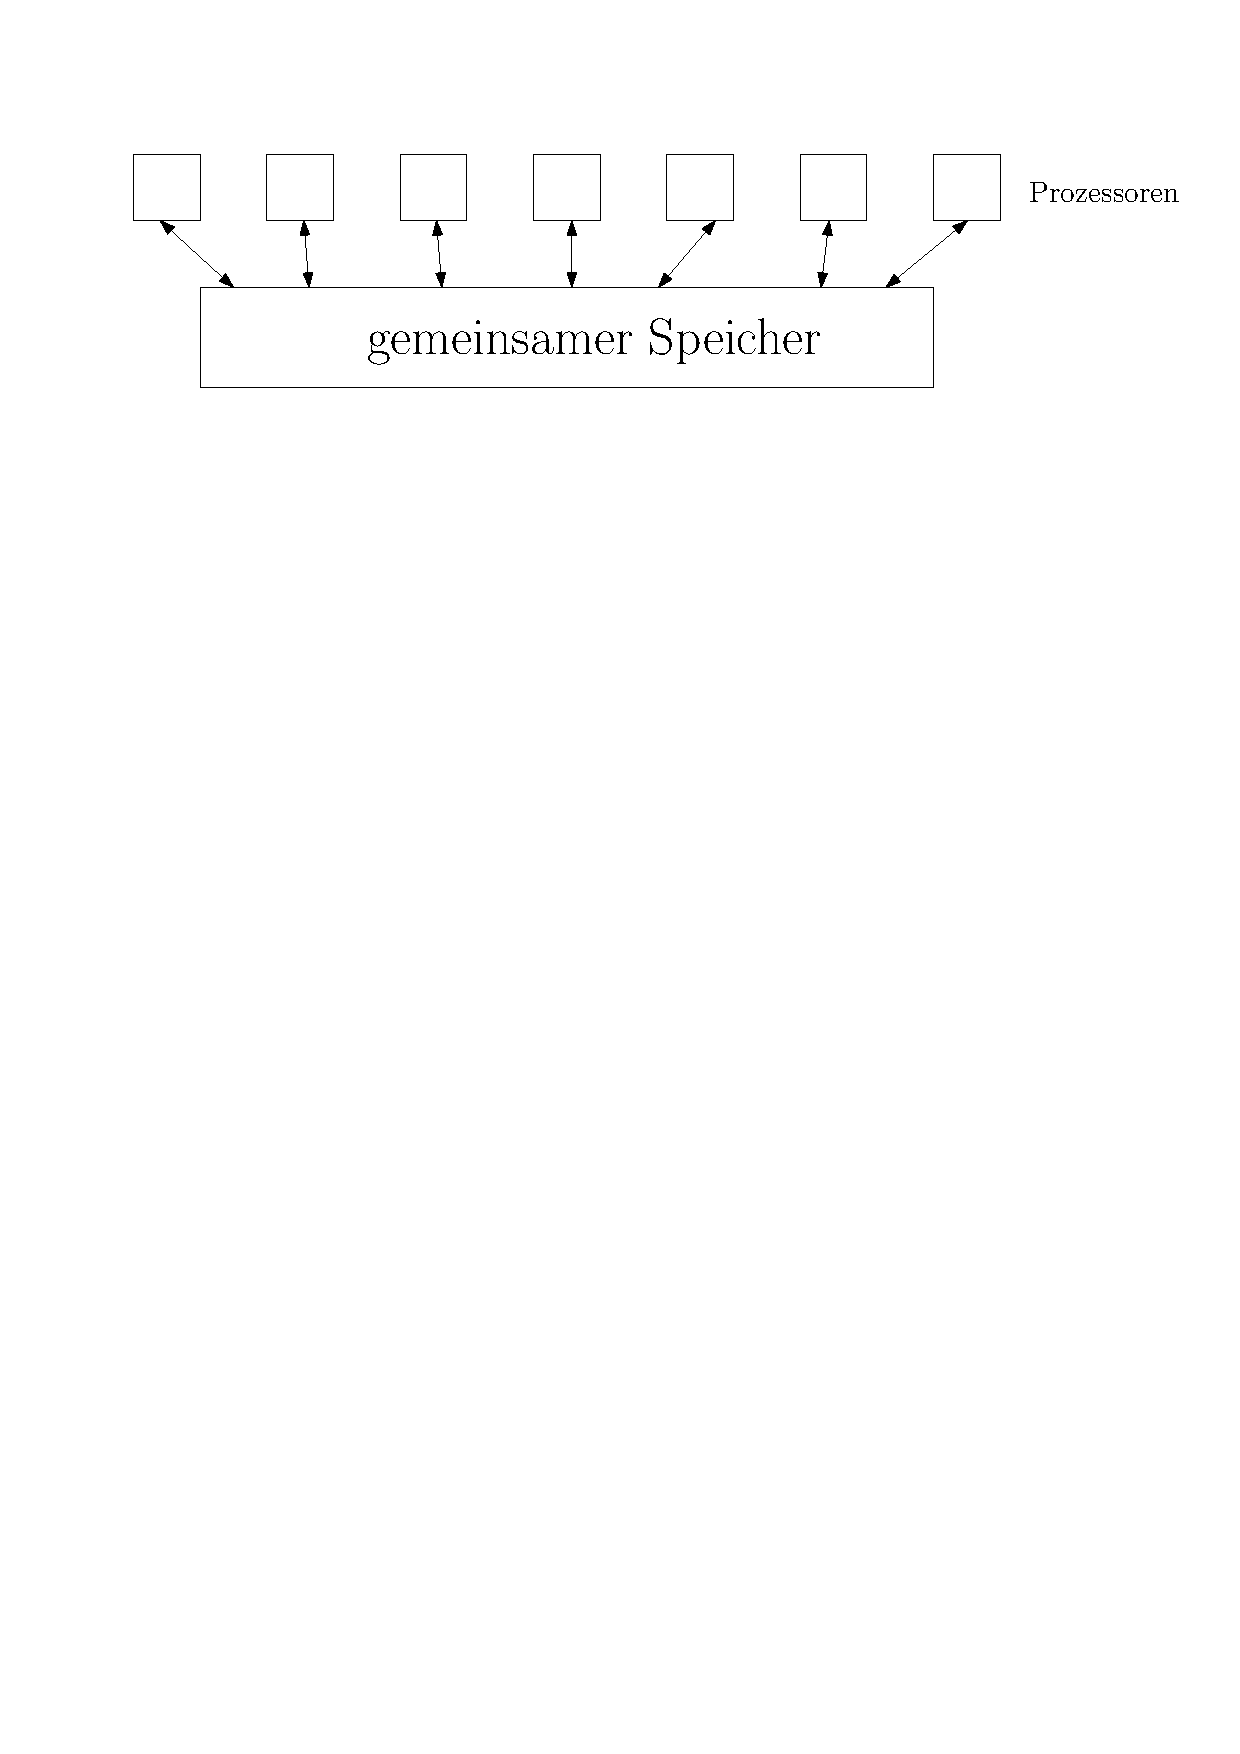
\includegraphics[scale=0.6]{bilder/PRAM.pdf}
\caption{Idee der parallelen Registermaschine}
\end{figure}

An der PRAM als Berechnungsmodell gab es die Kritik, dass die Anzahl der Prozessoren abhängig von der Eingabegröße sein darf und die PRAM somit kein realistisches Modell ist. Allerdings gilt das Gleiche bei der Registermaschine in Bezug auf den Speicherplatz. Trotz der Kritik wird die PRAM das Berechnungsmodell für die Analyse der Algorithmen sein, die in dieser Vorlesung vorgestellt werden, da sie die Möglichkeit einer größtmöglichen Parallelisierung eines Problems liefert. Eine Simulation mit weniger Prozessoren ist dann ggf. leicht zu bewerkstelligen. Außerdem ist sie als Modell für komplexe theoretische Betrachtungen sinnvoll und kann auch als Benutzerschnittstelle für parallele Programmierung dienen.

In den $1990\text{er}$ und $2000\text{er}$ Jahren wurde die Forschung auf dem Gebiet der parallelen Algorithmen und Architekturen fast eingestellt. Dies hatte mehrere Gründe. Aus theoretischer Sicht waren für viele Standardprobleme parallele Algorithmen entwickelt worden. In der Praxis wurden mehr Fortschritte durch die Beschleunigung der CPUs durch höhere Taktraten erreicht als durch die Entwicklung paralleler Architekturen. Außerdem war die bisherige Software historisch bedingt auf sequentielle Rechner ausgerichtet. Das Entwickeln und Erstellen paralleler Software war wesentlich schwieriger und teurer.

Heutzutage ist fast jeder Rechner ein Parallelrechner mit mehreren Kernen (cores). Graphikkarten sind ''special purpose hardware`` und arbeiten parallel. Die Firma NVIDIA entwickelte die Programmiersprache CUDA mit der parallele Algorithmen programmiert und auf Graphikkarten ausgeführt werden können.

In dieser Vorlesung wird CILK für die Implementierung paralleler Algorithmen verwendet, welches auf C bzw. C++ basiert. 

\section{Drei Beispiele paralleler Algorithmen}
\subsection{Berechnung der Summe von $n$ Zahlen.}
{\bf{Gegeben:}} $n$ Zahlen $a_1,\ldots,a_{n}$\\
{\bf{Berechne:}} $\sum_{i=1}^{n}{a_i}$\\
\\
Werden die $n$ Zahlen sequentiell aufaddiert wird $\Theta(n)$ Zeit benötigt. Angenommen, es stehen hinreichend viele Prozessoren zu Verfügung, die parallel arbeiten können, wie schnell kann das Problem dann gelöst werden? Wird die Summe in einer Art Baumstruktur berechnet, wobei auf jeder Ebene des Baumes die Operationen parallel ausgeführt werden, so kann die Summe von $n$ Zahlen in $O(\log n)$ Zeit mit $\frac{n}{2}$ Prozessoren berechnet werden.
\begin{figure}[h!]
\centering
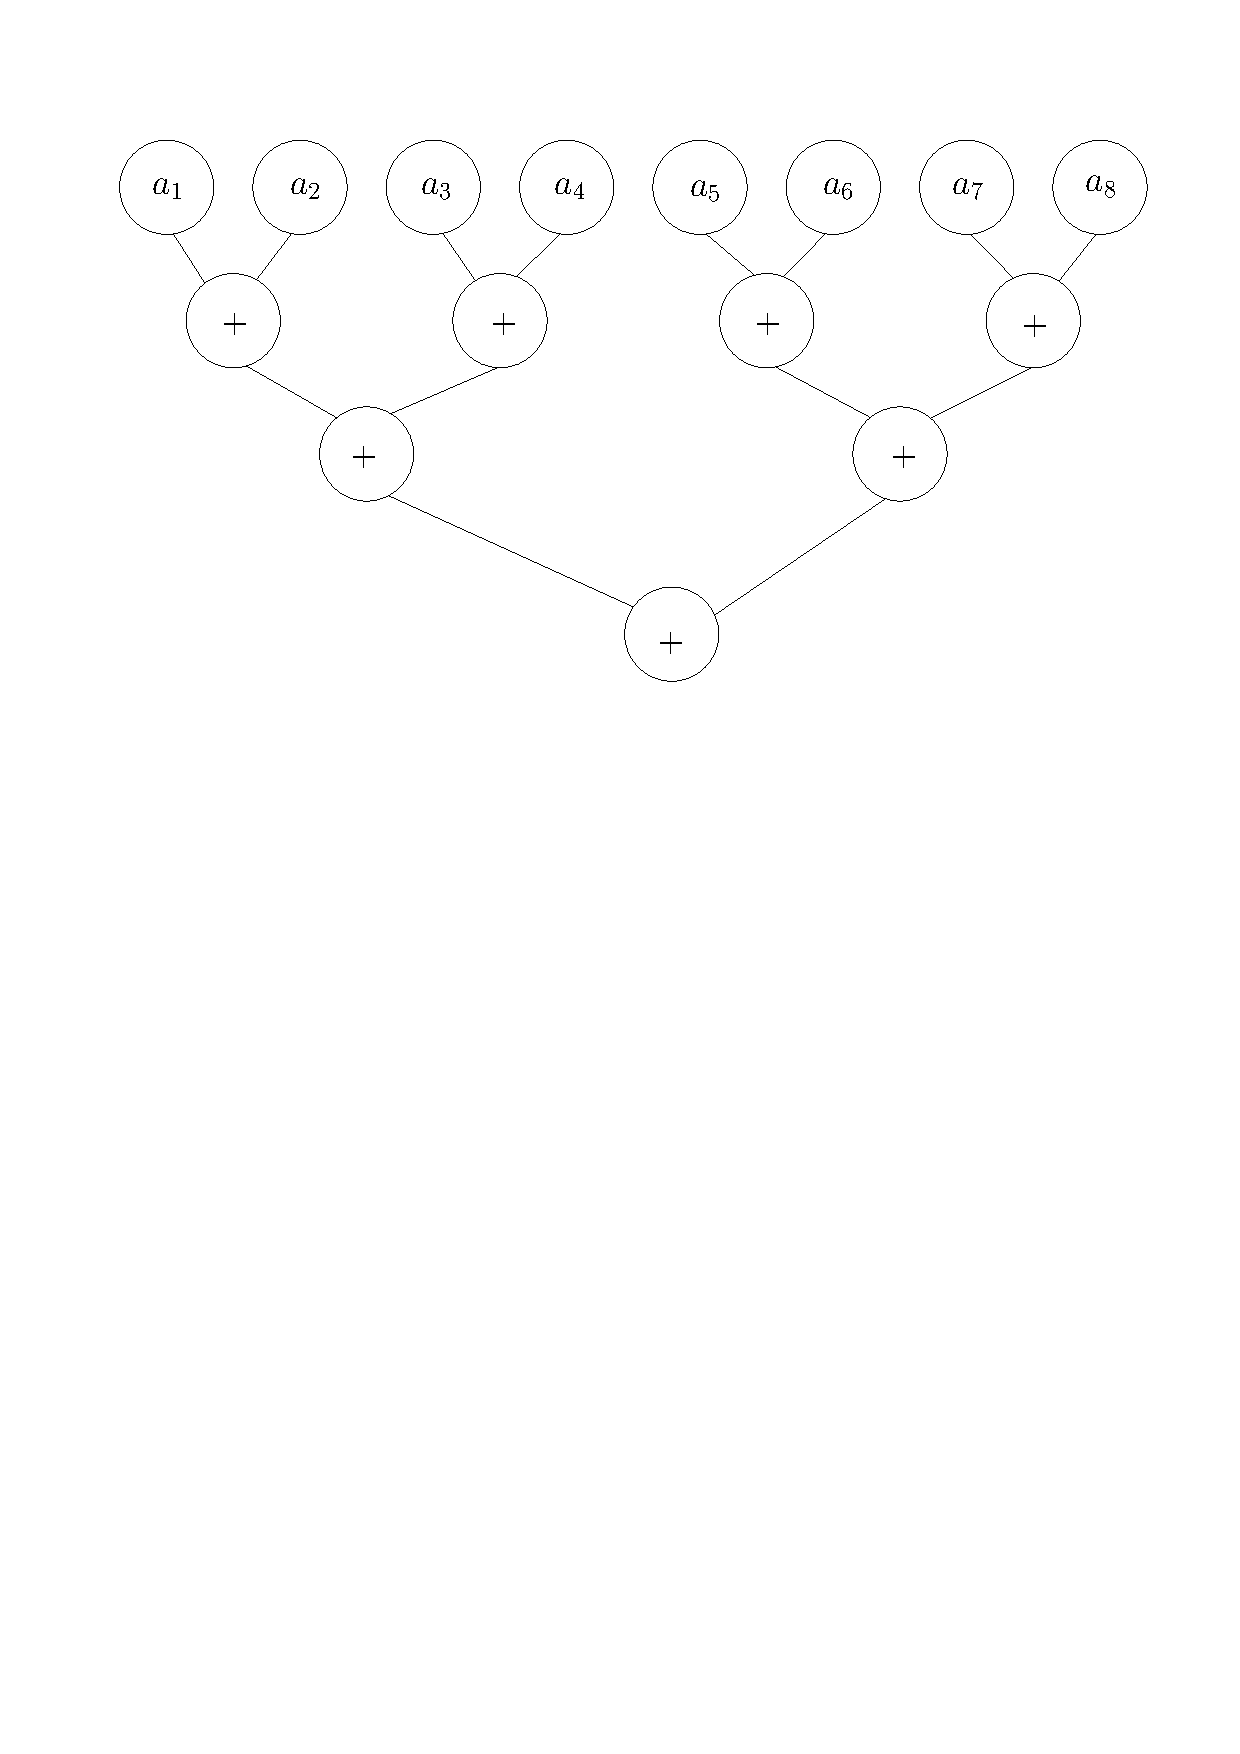
\includegraphics[scale=0.8]{bilder/SummeParallel.pdf}
\caption{Schema zur parallelen Berechnung der Summe von $n$ Zahlen.}
\end{figure}

Der Gesamtaufwand eines parallelen Algorithmus berechnet sich als das Produkt der Laufzeit und der Anzahl der Prozessoren. In diesem Fall wäre der Gesamtaufwand also $O(n\log n)$. Dies kann verbessert werden, indem nicht $\Theta(n)$ sondern $\Theta\left(\frac{n}{\log n}\right)$ viele Prozessoren verwendet werden. Die Folge der Zahlen wird zunächst in Blöcke der Größe $\Theta(\log n)$ unterteilt und die Summe jedes Blocks wird von einem Prozessor sequentiell berechnet. Dies braucht insgesamt $\Theta(\log n)$ Zeit für alle Summen, da die Prozessoren parallel arbeiten. Dann wird die Summe der $\Theta\left(\frac{n}{\log n}\right)$ Zahlen wie oben beschrieben parallel berechnet. Die Laufzeit ist $\Theta(\log n)$ und damit ist der Gesamtaufwand $\Theta\left(\frac{n}{\log n}\log n\right)=\Theta\left(n\right)$. \\
Algorithmus \ref{AlgSumNZahlen} beschreibt das vorgestellten Verfahren mit Hilfe von Pseudocode. Das Schlüsselwort \algpar bezeichnet die parallele Ausführung der Anweisungen in der zugehörigen Schleife.
\\
\begin{algorithm}
\caption{Summe der Zahlen $A[0],\ldots,A[n-1]$}
\label{AlgSumNZahlen}
\begin{algorithmic}[1]
\FOR {$h:=0$ \algto $\log n$}
\FOR {$i:=0$ \algstep $2^{h+1}$ \algto $n-2^{h+1}$ \algpar}
\STATE $A[i]:= A[i]+A[i+2^h]$;
\ENDFOR
\ENDFOR
\RETURN $A[0]$;
\end{algorithmic}
\end{algorithm}

Um die Summe von $n$ Zahlen zu berechnen, kann auch ein divide-\&-conquer Ansatz verwendet werden, der parallelisiert werden kann. In CILK und in unserem Pseudocode wird dazu der Befehl \algspawn vor den rekusiven Aufruf der Funktion geschrieben.
\\
\begin{algorithm}[h]
\caption{Summe der Elemente in $A$ mit divide-\&-conquer.}
\label{AlgSumNZahlenDC}
\begin{algorithmic}
\STATE {\bf{function add }}$(A,l,r)$
\IF {$l=r$} 
\RETURN $A[l]$;
\ELSE
\IF {$l<r$}
\STATE $m:=\lfloor{\frac{l+r}{2}}\rfloor$;
\STATE $x:=$\algspawn{\bf{add }}$(A,l,m)$;
\STATE $y:=$\algspawn{\bf{add }}$(A,m+1,r)$;
\RETURN $x+y$;
\ELSE
\RETURN $0$;
\ENDIF
\ENDIF
\end{algorithmic}
\end{algorithm}
\\
\\
\\
{\bf{Laufzeit }}(bei hinreichend vielen Prozessoren):\\
Sei $n = r-l+1$.
\begin{eqnarray*}
T(1) & = & c_1 \\
T(n) & = & T\left(\left\lceil\frac{n}{2}\right\rceil\right)+c_2,
\end{eqnarray*} für Konstanten $c_1$ und $c_2$.\\
Wegen der Parallelität wird das Maximum der Laufzeiten der beiden rekursiven Aufrufe betrachtet und nicht wie sonst die Summe der Laufzeiten.\\
Die Lösung der Rekursionsgleichung und somit die Laufzeit der Funktion {\bf{add}} ist $T(n)= O(\log n)$ mit $O(n)$ Prozessoren.
\\
\\
{\bf{Bemerkung:}} Der Algorithmus kann nicht nur für die Addition verwendet werden, sondern funktioniert für beliebige assoziative Operationen.
\subsection{Berechnung von Präfixsummen}
Als nächstes Beispiel betrachten wir die Berechnung der Präfixsummen von einer Folge von $n$ Zahlen. \\
{\bf{Gegeben:}} $n$ Zahlen $a_1,\ldots, a_n$\\
{\bf{Berechne:}} $n$ Zahlen $s_1,\ldots, s_n$ mit $s_k = \sum_{i=1}^{k}{a_i}$\\
\\
{\bf{Beispiel:}}\\
$\begin{matrix}
a: & 2 & 5 & 6 & 1 & 2 & 3 & 5 & 4\\
s: & 2 & 7 & 13 & 14 & 16 & 19 & 24 & 28
\end{matrix}$
\\
Ein einfacher sequentieller Algorithmus arbeitet wie folgt:
\begin{algorithm}
\caption{Sequentielles Berechnen der Präfixsummen.}
\label{AlgPSSeq}
\begin{algorithmic}
\STATE $s_0:=0$
\FOR{i:=1 \algto n}
\STATE $s_i:=s_{i-1}+a_i$;
\ENDFOR
\end{algorithmic}
\end{algorithm}
\\
{\bf{Laufzeit:}} Jede Schleifeniteration benötigt $\Theta(1)$ Zeit, somit ist die Gesamtlaufzeit $\Theta(n)$.\\
Algorithmus \ref{AlgPSSeq} lässt sich nicht einfach durch das Hinzufügen der Anweisung \algpar parallelisieren, da die jeweiligen Ergebnisse der  Berechnung in der Schleife nicht voneinander unabhängig sind.
\clearpage
Eine Möglichkeit eines parallelen Verfahrens zur Berechnung der Präfixsummen ist durch das folgende Schema gegeben:\\
\begin{figure}[h!]
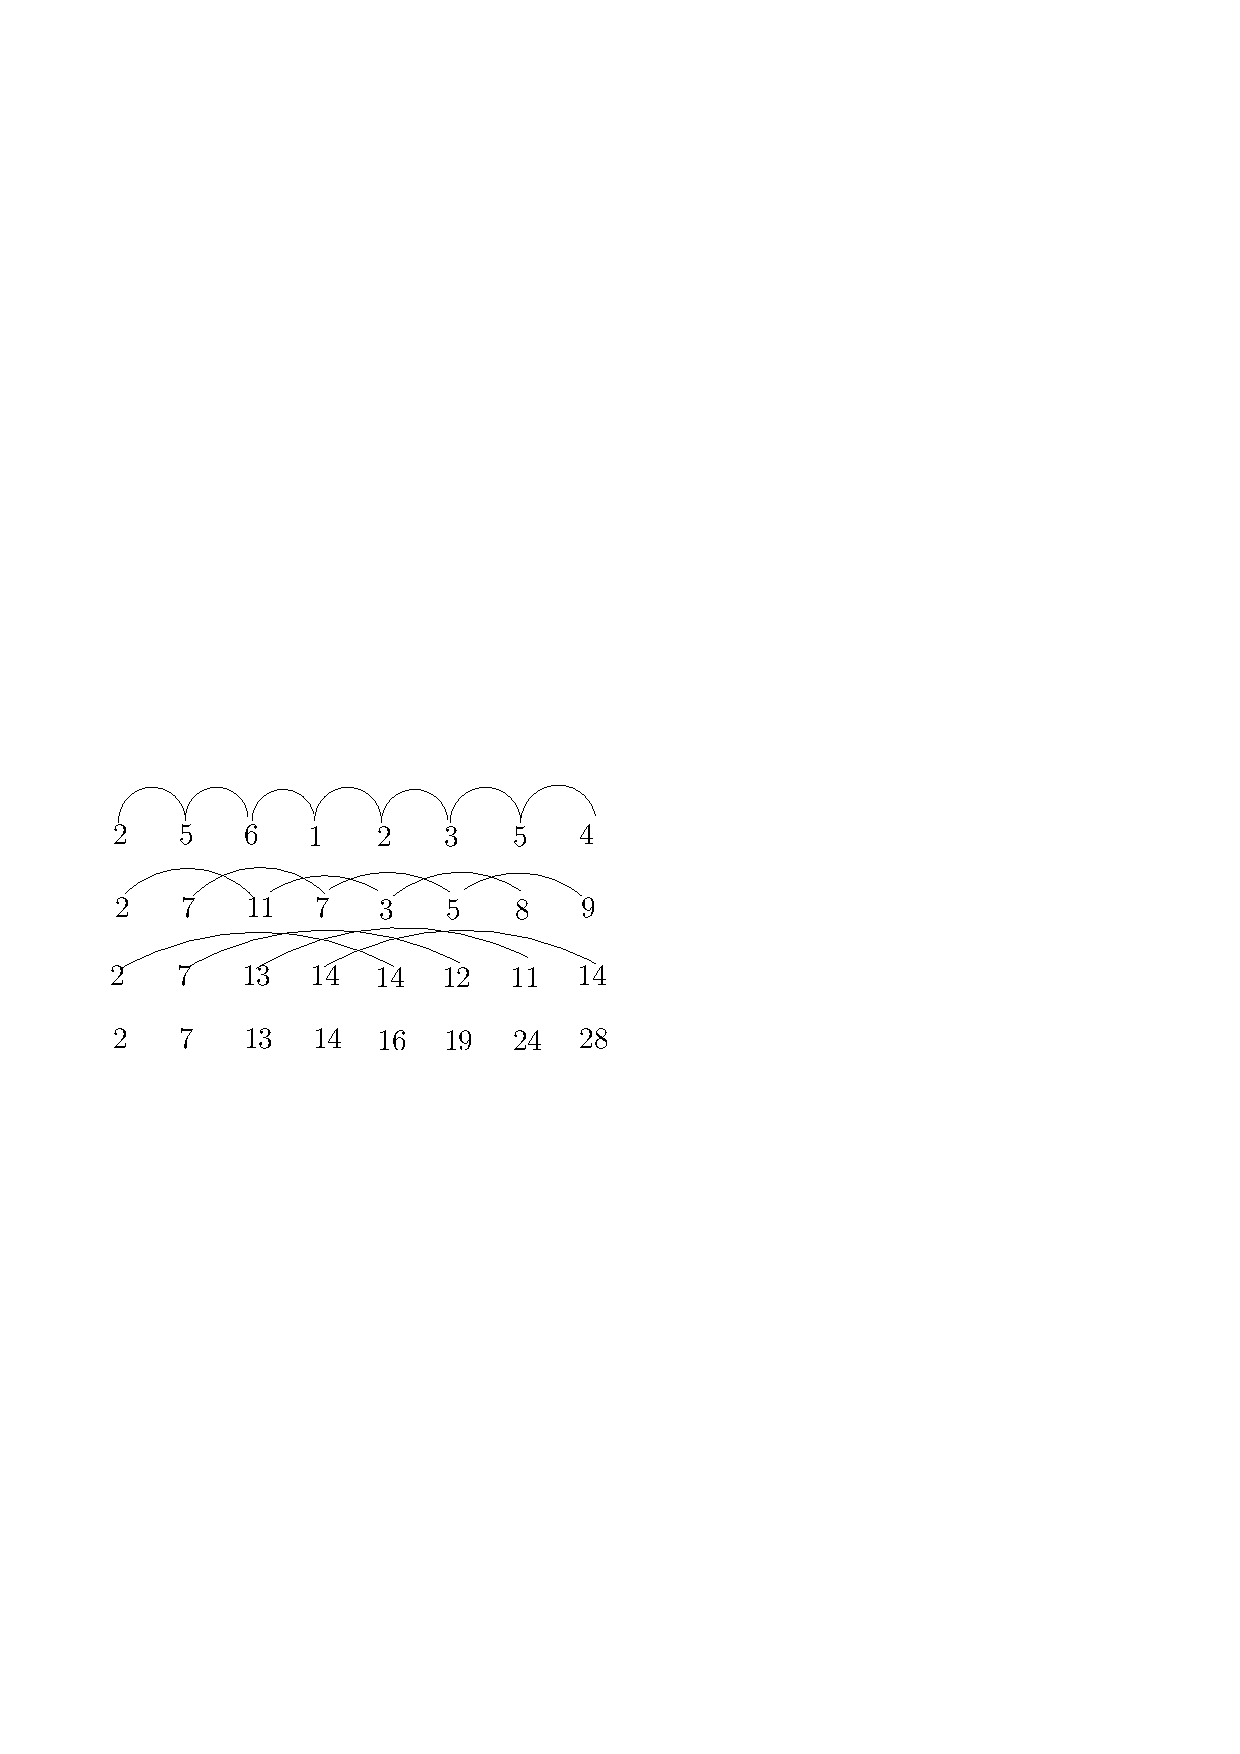
\includegraphics[scale=0.8]{bilder/PraefixsummeSchema.pdf}
\end{figure}
\\
Im ersten Schritt wird die Summe zweier in der Folge benachbarter Zahlen berechnet und an der Stelle der 2.~Zahl gespeichert. In den darauf folgenden Schritten werden jeweils die Summen zweier Zahlen mit Abstand zwei, vier, acht, etc. berechnet, bis im letzten Schritt die Summen zweier Zahlen mit Abstand $\frac{n}{2}$ berechnet werden. Diese bilden dann das Ergebnis der Präfixsummenfolge.
\begin{algorithm}[h!]
\caption{Paralleles Berechnen der Präfixsummen.}
\begin{algorithmic}
\STATE $h:=1$;
\FOR{$i:=1$ \algto $n$ \algpar}
\STATE $s_i:=a_i$;
\ENDFOR
\WHILE {$h\leq \frac{n}{2}$}
\FOR{$i:= h+1$ \algto $n$ \algpar}
\STATE $t_i:=s_i+s_{i-h}$;
\ENDFOR
\STATE $h:=h\cdot 2$;
\FOR{$i:=1$ \algto $n$ \algpar}
\STATE $s_i:=t_i$;
\ENDFOR
\ENDWHILE
\end{algorithmic}
\end{algorithm}
\\
\\
{\bf{Laufzeit:}} Da die Anweisungen in den for-Schleifen parallel ausgeführt werden, und zusammen $\Theta(1)$ Zeit benötigen, ist die Gesamtlaufzeit proportional zu der Anzahl der Schleifendurchläufe der while-Schleife. Diese wird $\Theta(\log n)$ mal durchlaufen, da $h$  bei jedem Durchlauf verdoppelt wird. Die Laufzeit des parallelen Algorithmus' zur Berechnung der Präfixsummen von $n$ Zahlen ist somit $\Theta(\log n)$ mit $n$ Prozessoren.
